\documentclass[aspectratio=169,10pt]{beamer}

\usetheme{default}
\setbeamertemplate{navigation symbols}{}
\setbeamertemplate{footline}{%
  \hfill\usebeamerfont{page number in head/foot}\insertframenumber/\inserttotalframenumber\hspace{1.2em}\vspace{0.8em}
}
\setbeamertemplate{itemize item}{\raise0.2ex\hbox{\scriptsize$\blacktriangleright$}}
\setbeamertemplate{itemize subitem}{\raise0.2ex\hbox{\scriptsize$\triangleright$}}

\usepackage[T1]{fontenc}
\usepackage{lmodern}
\usepackage{amsmath,amssymb,booktabs,array,multirow}
\usepackage{graphicx}
\usepackage{tikz}
\usepackage[numbers,sort&compress]{natbib}
\providecommand{\doi}[1]{}
\usetikzlibrary{arrows.meta,positioning,calc}

\definecolor{ink}{RGB}{22,31,45}
\definecolor{slate}{RGB}{48,61,78}
\definecolor{muted}{RGB}{94,105,118}
\definecolor{rulegray}{RGB}{190,196,204}
\definecolor{deepblue}{RGB}{18,52,86}
\definecolor{wine}{RGB}{124,36,45}
\definecolor{forest}{RGB}{34,93,73}
\definecolor{paper}{RGB}{250,250,248}

\setbeamercolor{normal text}{fg=ink,bg=paper}
\setbeamercolor{frametitle}{fg=deepblue,bg=paper}
\setbeamercolor{title}{fg=deepblue}
\setbeamercolor{subtitle}{fg=slate}
\setbeamercolor{structure}{fg=deepblue}
\setbeamercolor{alerted text}{fg=wine}
\setbeamerfont{title}{series=\bfseries,size=\Large}
\setbeamerfont{frametitle}{series=\bfseries,size=\large}
\setbeamerfont{author}{size=\normalsize}
\setbeamerfont{date}{size=\small}
\setbeamerfont{jointwork}{size=\scriptsize}

\setlength{\parskip}{0.25em}
\renewcommand{\arraystretch}{1.18}

\newcommand{\E}{\mathbb{E}}
\newcommand{\Pbb}{\mathbb{P}}
\newcommand{\one}{\mathbf{1}}
\newcommand{\surv}{p_{\mathrm{surv}}}
\newcommand{\liq}{p_{\mathrm{liq}}}
\newcommand{\hf}{H}

\title[A semi-analytic framework for DeFi long--short sizing]{A semi-Analytic Framework for Long--Short Position Sizing in DeFi under Liquidation and Jump Risk}
\author{Francis Liu}
\institute{Academic hour}
\date{30th June 2026}

\begin{document}

% ------------------------------------------------------------
\begin{frame}
  \vspace{1.0em}
  {\usebeamerfont{title}\usebeamercolor[fg]{title}\inserttitle\par}
  \vspace{1.2em}
  {\usebeamerfont{author}\insertauthor\par}
  \vspace{0.7em}
  {\usebeamerfont{jointwork}
    Joint work with Professor Daniel Pele, Department of Statistics and Econometrics,\\
    Bucharest University of Economic Studies\\
    Theodor Ginavar, PhD Candidate, MSCA Digital Finance\par}
  {\usebeamerfont{date}\insertinstitute\hspace{0.6em}|\hspace{0.6em}\insertdate\par}
  \vfill
  \begin{center}
    
\begin{tikzpicture}
      \draw[deepblue,very thick] (0,0) -- (10.8,0);
      \draw[wine,thick] (0,-0.12) -- (2.4,-0.12);
    \end{tikzpicture}
  \end{center}
  \vspace{0.8em}
  \large DeFi long--short sizing under liquidation and jump risk
\end{frame}

% ------------------------------------------------------------
\begin{frame}{DeFi Lending Platforms}
  \small
  Aave / Compound: pooled lending
  \vspace{0.4em}

  \begin{itemize}
    \item \textbf{Mechanism} lenders supply pool assets; borrowers draw pooled liquidity
    \item \textbf{Accounting} no bilateral lender; protocol-level collateral and debt balances
    \item \textbf{Interest accrual} variable supply/borrow APRs; utilization-driven index growth
    \item \textbf{No fixed tenor} open-ended loans; no maturity date; no term structure contract
  \end{itemize}

  \vspace{0.25em}
  \textbf{Overcollateralization}
  \begin{itemize}
    \item Pseudonymous parties; no credit underwriting; no legal margin call
    \item Solvency and obligation enforcement entirely collateral-based
    \item No-arbitrage discipline through collateral constraint
    \item \textbf{Liquidator role} repay unsolvent debt; seize collateral bonus; restore pool solvency
  \end{itemize}

\end{frame}

% ------------------------------------------------------------
\begin{frame}{Health Factor and Boundary}
  \small
  {\bf{Key mechanism variables}}
  \vspace{0.35em}

  State variables:
  \[
    V_{1,t}:=n_1S_{1,t}\quad\text{collateral value},
    \qquad
    V_{2,t}:=n_2S_{2,t}\quad\text{borrow/debt value}
  \]
  \vspace{0.25em}

  Loan-to-value* and liquidation threshold:
  \[
    \mathrm{LTV}_t:=\frac{V_{2,t}}{V_{1,t}},
    \qquad
    b=\mathrm{threshold\ LTV}
  \]
  Aave origination LTV $<$ threshold LTV $b$; initial buffer by design
  \vspace{0.25em}

  Health factor:
  \[
    H_t:=\frac{b\,V_{1,t}}{V_{2,t}}
    =
    \frac{b}{\mathrm{LTV}_t}
  \]
  \vspace{0.25em}

  Liquidation triggering condition:
  \[
    H_t<1
    \quad\Longleftrightarrow\quad
    V_{2,t}>b\,V_{1,t}
  \]

  {\scriptsize * Remark: for now, ignore origination-LTV / threshold-LTV gap}
  \vspace{0.2em}
\end{frame}

% ------------------------------------------------------------
\begin{frame}{Constructing the Long--Short Position}
  \begin{center}
    \begin{tabular}{@{}p{0.15\linewidth}p{0.45\linewidth}p{0.30\linewidth}@{}}
      \toprule
      Step & Protocol action & Economic exposure \\
      \midrule
      0 & Initial capital injection: \$1-worth BTC & External capital only \\
      1 & Supply BTC collateral to Aave & Long BTC collateral \\
      2 & Borrow \$0.8-worth ETH & Short ETH liability \\
      3 & Sell ETH into \$0.8-worth BTC & Self-financing conversion \\
      4 & Re-supply BTC as collateral & Total BTC collateral: \$1.8 \\
      \midrule
      Result & Collateralized debt position & Leveraged long BTC, short ETH \\
      \bottomrule
    \end{tabular}
  \end{center}
  \vspace{0.55em}
  Resulting normalized position:
  \begin{itemize}
    \item External capital: \$1; no additional capital after step 0
    \item BTC collateral: \$1.8; ETH debt: \$0.8
    \item $b=0.8$; $H_0=0.8\times1.8/0.8=1.8$
    \item Leveraged BTC exposure; short ETH exposure
  \end{itemize}
\end{frame}

% ------------------------------------------------------------
\begin{frame}{Looping the Position}
  \small
  Repeat steps 1--4; zero transaction cost and slippage
  \vspace{0.35em}

  Round-$m$ additional collateral:
  \[
    1,\quad b,\quad b^2,\quad \ldots,\quad b^m
  \]
  Total BTC collateral after $m$ loops:
  \[
    V_1^{(m)}
    =
    1+b+\cdots+b^m
    =
    \frac{1-b^{m+1}}{1-b}
  \]
  ETH debt:
  \[
    V_2^{(m)}
    =
    b+b^2+\cdots+b^{m+1}
    =
    b\,V_1^{(m)}
  \]
  Infinite-loop limit:
  \[
    V_1^{(\infty)}=\frac{1}{1-b},
    \qquad
    V_2^{(\infty)}=\frac{b}{1-b}
  \]
  Example $b=0.8$:
  \[
    V_1^{(\infty)}=5,
    \qquad
    V_2^{(\infty)}=4,
    \qquad
    H_0^{(\infty)}=\frac{bV_1^{(\infty)}}{V_2^{(\infty)}}=1
  \]
  Extreme leverage: any adverse move $\rightarrow$ liquidation; favorable move $\rightarrow$ amplified gain
\end{frame}

% ------------------------------------------------------------
\begin{frame}{Unwinding and Taking Profit}
  \small
  Favorable scenario: BTC $+10\%$; ETH $-16.7\%$
  \[
    H_t=\frac{0.80\,V_{1,t}}{V_{2,t}},
    \qquad
    \text{equity}=V_{1,t}-V_{2,t}
  \]
  \vspace{0.15em}
  \begin{center}
    \begin{tabular}{@{}p{0.17\linewidth}r r c r p{0.20\linewidth}@{}}
      \toprule
      Scenario & BTC collat. & ETH debt & $H$ & Equity & Action \\
      \midrule
      Entry & \$1.80 & \$0.80 & $1.80$ & \$1.00 & Hold \\
      Favorable move & \$1.98 & \$0.667 & $2.38$ & \$1.313 & Voluntary unwind \\
      \bottomrule
    \end{tabular}
  \end{center}
  \vspace{0.5em}
  Outcome:
  \[
    \text{gain}=1.313-1.000=0.313
  \]
  Voluntary unwind; solvent position; profit realization
\end{frame}

% ------------------------------------------------------------
\begin{frame}{Aave Liquidation and Immediate Risk}
  \small
  Adverse scenario: BTC $-25\%$; ETH $+40\%$
  \[
    H_t=\frac{bV_{1,t}}{V_{2,t}}
    =
    \frac{0.80\,V_{1,t}}{V_{2,t}},
    \qquad
    H_t\leq1
    \Longleftrightarrow
    \frac{V_{2,t}}{V_{1,t}}\geq0.80
  \]
  \vspace{0.15em}
  \begin{center}
    \begin{tabular}{@{}p{0.17\linewidth}r r c r p{0.20\linewidth}@{}}
      \toprule
      Scenario & BTC collat. & ETH debt & $H$ & Equity & Outcome \\
      \midrule
      Entry & \$1.80 & \$0.80 & $1.80$ & \$1.00 & Safe \\
      Adverse move & \$1.35 & \$1.12 & $0.96$ & \$0.23 & Liquidatable \\
      \bottomrule
    \end{tabular}
  \end{center}
  \vspace{0.35em}
  Outcome:
  \[
    H_t<1
    \quad\Rightarrow\quad
    \text{keeper liquidation; collateral seized at bonus}
  \]
  Recovery drivers: shock severity; market sentiment/liquidity; liquidator inventory willingness; gas fees
  \vspace{0.2em}

  Modeling convention: detailed recovery omitted; $\Pi_T=0$ whenever $\tau\le T$
\end{frame}

% ------------------------------------------------------------
\begin{frame}{Payoff Function from the Trade}
  \small
  Holdings: $n_1$ units of collateral asset $S_1$; debt: $n_2$ units of borrowed asset $S_2$
  \vspace{0.3em}

  Surviving-path terminal wealth:
  \[
    \Pi_T:=(n_1S_{1,T}-n_2S_{2,T})\,\one_{\{\tau>T\}}
  \]
  Running BTC/ETH example:
  \[
    S_1=\mathrm{BTC},\qquad S_2=\mathrm{ETH},
    \qquad n_1S_{1,0}=1.80,\qquad n_2S_{2,0}=0.80
  \]
  Therefore:
  \[
    \Pi_T=
    \left(
      1.80\,\frac{S_{1,T}}{S_{1,0}}
      -
      0.80\,\frac{S_{2,T}}{S_{2,0}}
    \right)\one_{\{\tau>T\}}
  \]
  Survival indicator: $\tau\le T \Rightarrow \Pi_T=0$
  \vspace{0.25em}

  Initial net book value normalized to one unit of account; moments stated directly in $\Pi_T$
\end{frame}

% ------------------------------------------------------------
\begin{frame}{Why Payoff Moments Are Hard}
  \small
  Target statistics:
  \[
    \E[\Pi_T],\qquad
    \mathrm{Var}(\Pi_T),\qquad
    \E[\Pi_T^k],\quad k\ge1
  \]
  Killed payoff:
  \[
    \Pi_T^k
    =
    (n_1S_{1,T}-n_2S_{2,T})^k
    \one_{\{\tau>T\}}
  \]
  Terminal payoff state:
  \[
    (S_{1,T},S_{2,T})
  \]
  Pathwise killing process:
  \[
    \tau>T
    \quad\Longleftrightarrow\quad
    H_s\ge1\ \text{ for all }s\le T,
    \qquad
    H_s=\frac{b\,n_1S_{1,s}}{n_2S_{2,s}}
  \]
  Direct moment:
  \[
    \E_\Pbb[\Pi_T^k]
    =
    \E_\Pbb\!\left[(n_1S_{1,T}-n_2S_{2,T})^k\one_{\{\tau>T\}}\right]
  \]
  Difficulty: terminal bivariate payoff + pathwise barrier
  \vspace{0.25em}

  Generic numerical routes:
  \begin{itemize}
    \item Monte Carlo; barrier monitoring / possible 2D Brownian-bridge refinement
    \item Numerical PDE/PIDE; two terminal state variables plus killing boundary
  \end{itemize}
\end{frame}

% ------------------------------------------------------------
\begin{frame}{Literature Positioning}
  \small
  Intersection:
  \[
    \text{DeFi liquidation}
    \quad+\quad
    \text{first-passage methods for jump diffusions}
  \]
  \vspace{0.35em}

  \begin{itemize}
    \item \textbf{DeFi liquidation} Qin et al.~\cite{Qin2021}; Heimbach--Huang~\cite{HeimbachHuang2024}
    \item Incentive structure; leverage amplification; liquidation cascades
    \item Empirical focus; no ex-ante sizing rule
  \end{itemize}
  \vspace{0.25em}

  \begin{itemize}
    \item \textbf{First passage under jumps} Kou--Wang~\cite{KouWang2003}; Sepp~\cite{Sepp2004}
    \item Double-exponential jumps; Laplace transforms; finite algebraic systems
    \item Classical object: single-asset barrier option
  \end{itemize}
  \vspace{0.25em}

  Gap:
  \[
    \text{barrier-killed long--short ratio}
    \quad\neq\quad
    \text{single-asset barrier option}
  \]
  Bridge: change of measure $\rightarrow$ one-dimensional killed expectation
\end{frame}

% ------------------------------------------------------------
\begin{frame}{Price Process}
  \small
  Jump motivation: crypto gaps; flash crashes; barrier crossed before rebalance
  \hfill Kou model~\cite{Kou2002}
  \vspace{0.25em}

  Price dynamics, $i=1,2$:
  \[
    S_{i,t}=S_{i,0}e^{X_{i,t}},
    \qquad
    dX_{i,t}
    =
    \mu_i^X\,dt+\sigma_i\,dB_{i,t}
    +d\!\left(\sum_{n=1}^{N_{i,t}}J_i^{(n)}\right)
  \]
  Brownian correlation:
  \[
    d\langle B_1,B_2\rangle_t=\rho\,dt,
  \]
  Poisson intensity: $\lambda_i$
  \vspace{0.2em}

  Kou double-exponential jump density:
  \[
    f_i(j)
    =
    \frac{p_i}{\eta_{i,+}}e^{-j/\eta_{i,+}}\one_{\{j>0\}}
    +
    \frac{1-p_i}{\eta_{i,-}}e^{j/\eta_{i,-}}\one_{\{j<0\}}
  \]
  Drift normalization: $\E_\P[S_{i,t}/S_{i,0}]=e^{\mu_i t}$
  \[
    \mu_i^X=\mu_i-\frac12\sigma_i^2-\lambda_i\chi_i,
    \qquad
    \chi_i=\E[e^{J_i}-1]
    =
    \frac{p_i}{1-\eta_{i,+}}+\frac{1-p_i}{1+\eta_{i,-}}-1
  \]
  Constant supply/borrow rates absorbed into drift; dynamic rate modeling outside scope
\end{frame}

% ------------------------------------------------------------
\begin{frame}{Semi-Analytic Architecture}
  \small
  \begin{center}
    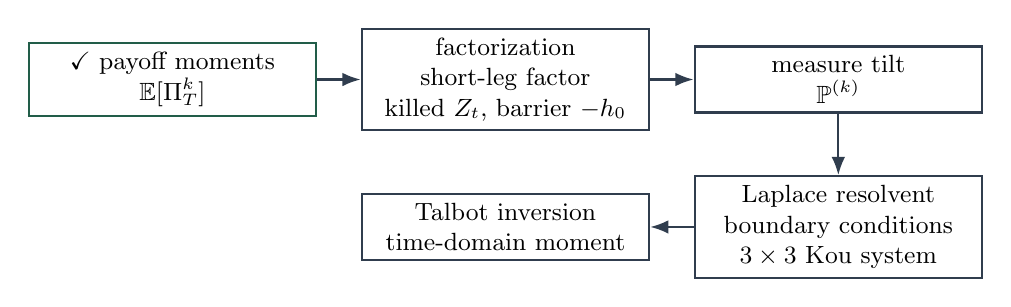
\begin{tikzpicture}[
      stage/.style={draw=slate,thick,minimum width=3.65cm,minimum height=0.82cm,align=center,font=\small},
      done/.style={draw=forest,thick,minimum width=3.65cm,minimum height=0.82cm,align=center,font=\small},
      arr/.style={-Latex,thick,slate}
    ]
      \node[done] (a) {$\checkmark$ payoff moments\\$\E[\Pi_T^k]$};
      \node[stage,right=0.55cm of a] (b) {factorization\\short-leg factor\\killed $Z_t$, barrier $-h_0$};
      \node[stage,right=0.55cm of b] (c) {measure tilt\\$\Pbb^{(k)}$};
      \node[stage,below=0.78cm of c] (d) {Laplace resolvent\\boundary conditions\\$3\times3$ Kou system};
      \node[stage,left=0.55cm of d] (e) {Talbot inversion\\time-domain moment};
      \draw[arr] (a) -- (b);
      \draw[arr] (b) -- (c);
      \draw[arr] (c) -- (d);
      \draw[arr] (d) -- (e);
    \end{tikzpicture}
  \end{center}
  \vspace{0.45em}
  Covered: payoff function + need for moments
  \vspace{0.25em}

  Next: factorization and measure change $\rightarrow$ one-dimensional killed expectation
  \[
    k\,\eta_{2,+}<1
    \quad\text{moment-admissibility condition}
  \]
\end{frame}

% ------------------------------------------------------------
\begin{frame}{Factorization: From Two Assets to One Barrier}
  \small
  Motivation: separate terminal short-leg factor; isolate killed ratio problem
  \vspace{0.25em}

  Bivariate payoff; scalar liquidation state:
  \[
    Z_t=X_{1,t}-X_{2,t}
  \]
  Initial log health factor:
  \[
    h_0:=\log H_0
  \]
  Factorization using $H_T=e^{h_0+Z_T}$:
  \[
    \Pi_T
    =
    \frac{n_2}{b}\,S_{2,0}e^{X_{2,T}}
    (e^{h_0+Z_T}-b)\,\one_{\{\tau>T\}}
  \]
  One-dimensional payoff kernel:
  \[
    g_k(z;h_0):=(e^{h_0+z}-b)^k,
  \]
  Integer moments:
  \[
  \begin{aligned}
    \Pi_T^k
    &=
    \underbrace{
      \Big(\frac{n_2}{b}\Big)^kS_{2,0}^k e^{kX_{2,T}}
    }_{\mathcal F_T^{S_2}\text{ part}}
    \underbrace{
      g_k(Z_T;h_0)\,\one_{\{\tau>T\}}
    }_{\mathcal F_T^{Z}\text{ killed-ratio part}}
  \end{aligned}
  \]
  Measure change: absorb $\mathcal F_T^{S_2}$ factor; retain killed expectation under $Z$
  \vspace{0.3em}

  Barrier-option analogue: scalar state $Z$, barrier $-h_0$
\end{frame}

% ------------------------------------------------------------
\begin{frame}{Measure Change}
  \scriptsize
  Start from factorized moment:
  \[
    \E_\Pbb[\Pi_T^k]
    =
    \Big(\frac{n_2}{b}\Big)^kS_{2,0}^k\,
    \E_\Pbb\!\left[
      e^{kX_{2,T}}g_k(Z_T;h_0)\one_{\{\tau>T\}}
    \right]
  \]
  Exponential tilt:
  \[
    \left.\frac{d\Pbb^{(k)}}{d\Pbb}\right|_{\mathcal F_T}
    =
    \frac{e^{kX_{2,T}}}{\E[e^{kX_{2,T}}]}
  \]
  Heuristic reminder, with $Y=g_k(Z_T;h_0)\one_{\{\tau>T\}}$:
  \[
  \begin{aligned}
    \E_{\Pbb^{(k)}}[Y]
    &=
    \int Y\,d\Pbb^{(k)}
    =
    \int Y\,\frac{d\Pbb^{(k)}}{d\Pbb}\,d\Pbb\\
    &=
    \E_\Pbb\!\left[
      Y\,\frac{e^{kX_{2,T}}}{\E_\Pbb[e^{kX_{2,T}}]}
    \right]
    &=
    \frac{\E_\Pbb[e^{kX_{2,T}}Y]}{\E_\Pbb[e^{kX_{2,T}}]}
    \quad\Longrightarrow\quad
    \E_\Pbb[e^{kX_{2,T}}Y]
    =
    \E_\Pbb[e^{kX_{2,T}}]\E_{\Pbb^{(k)}}[Y]
  \end{aligned}
  \]
  {\scriptsize Remark: Radon--Nikodym theorem / change-of-measure identity}
  \vspace{0.15em}

  Reduced moment:
  \[
    \E[\Pi_T^k]
    =
    \Big(\frac{n_2}{b}\Big)^kS_{2,0}^k
    \E[e^{kX_{2,T}}]\,
    \E^{(k)}\!\left[
      g_k(Z_T;h_0)\one_{\{\tau>T\}}
    \right]
  \]
  Bivariate payoff moment $\rightarrow$ killed expectation of the ratio process
\end{frame}

% ------------------------------------------------------------
\begin{frame}{Tilted Ratio Process}
  \small
  Remaining object:
  \[
    \E^{(k)}\!\left[
      g_k(Z_T;h_0)\one_{\{\tau>T\}}
    \right]
  \]
  Question:
  \[
    Z_t=X_{1,t}-X_{2,t}
    \quad\text{under}\quad \Pbb^{(k)}
  \]
  Under $\Pbb^{(k)}$: $Z$ remains a L\'evy process

  L\'evy--Khintchine exponent of $Z$ under $\Pbb^{(k)}$:
  \[
    \psi_Z^{(k)}(s)
    =
    \mu_Z^{(k)}s+\frac12\sigma_Z^2s^2
    +\lambda_1\big(M_1(s)-1\big)
    +\lambda_2\big(M_2(k-s)-M_2(k)\big)
  \]
  with
  \[
    M_i(s)=
    \frac{p_i}{1-s\eta_{i,+}}
    +
    \frac{1-p_i}{1+s\eta_{i,-}},
    \qquad
    \sigma_Z^2=\sigma_1^2+\sigma_2^2-2\rho\sigma_1\sigma_2
  \]
  $\mathcal L^{(k)}$: infinitesimal generator of $Z$ under $\Pbb^{(k)}$, the generator eigenrelation:
  \[
    \mathcal L^{(k)}e^{sz}=\psi_Z^{(k)}(s)e^{sz}
  \]
\end{frame}

% ------------------------------------------------------------
\begin{frame}{Killed Moment PIDE}
  \small
  Target function:
  \[
    U(t,z)
    :=
    \E_z^{(k)}\!\left[
      g_k(Z_t;h_0)\one_{\{\tau(h_0)>t\}}
    \right],
    \qquad z>-h_0
  \]
  \vspace{0.2em}

  Backward Kolmogorov PIDE for the killed process:
  \[
    \partial_t U(t,z)=\mathcal L^{(k)}U(t,z),
    \qquad z>-h_0
  \]
  Initial and absorbing boundary:
  \[
    U(0,z)=g_k(z;h_0),
    \qquad
    U(t,z)=0\quad\text{for }z\le -h_0
  \]
  \vspace{0.2em}
  
  One time variable; one state variable $z$ for the ratio process $Z$

\end{frame}

% ------------------------------------------------------------
\begin{frame}{Laplace Transform Trick}
  \small
  Time-domain PIDE:
  \[
    \partial_t U(t,z)=\mathcal L^{(k)}U(t,z),
    \qquad
    U(0,z)=g_k(z;h_0)
  \]
  Laplace transform in time:
  \[
    \widehat U(q,z)=\int_0^\infty e^{-qt}U(t,z)\,dt,
    \qquad q>0
  \]
  Laplace-domain resolvent:
  \[
    (q-\mathcal L^{(k)})\widehat U(q,z)=g_k(z;h_0),
    \qquad z>-h_0
  \]
  Sepp~\cite{Sepp2004} idea:

  Laplace transform $+$ double-exponential jumps $\rightarrow$ finite algebraic system
  \vspace{0.25em}

  Here:
  \[
    \psi_Z^{(k)}(\gamma)=q
    \quad\Longrightarrow\quad
    \text{degree-six characteristic equation}
  \]
  Three admissible roots $+$ three boundary conditions $\rightarrow 3\times3$ system
\end{frame}

% ------------------------------------------------------------
\begin{frame}{Resolvent Solution Form}
  \small
  Resolvent decomposition:
  \[
    \widehat U(q,z;h_0)
    =
    \widehat U_{\mathrm{part}}(q,z;h_0)
    +
    \widehat U_{\mathrm{hom}}(q,z;h_0)
  \]
  Particular solution:
  \[
    \widehat U_{\mathrm{part}}(q,z;h_0)
    =
    \sum_{j=0}^{k}
    \frac{c_{k,j}(h_0)}{q-\psi_Z^{(k)}(j)}e^{jz}
  \]
  Homogeneous solution:
  \[
    \widehat U_{\mathrm{hom}}(q,z;h_0)
    =
    \sum_{m=1}^{3}
    B_m^{(k)}(q;h_0)e^{\gamma_{m+3}(q)(z+h_0)}
  \]
  Boundary coefficients:
  \[
    \underbrace{\mathbf M_{\mathrm{bar}}^{(k)}(q)}_{3\times3}
    \underbrace{\mathbf B^{(k)}}_{3\times1}
    =
    -\underbrace{\mathbf b^{(k)}}_{3\times1}
  \]
  PIDE solve $\rightarrow$ summation of exponentials $+$ one $3\times3$ linear system
\end{frame}

% ------------------------------------------------------------
\begin{frame}{Numerical Example}
  \scriptsize
  Conditional statistics; Laplace--resolvent vs MC survival
  \vspace{0.15em}

  \begin{center}
  \resizebox{0.84\textwidth}{!}{%
  \begin{tabular}{cc cc cccc}
  \toprule
  $h_0$ & $H_0$ & $p_{\mathrm{surv}}^{\mathrm{Lap}}$ & $p_{\mathrm{surv}}^{\mathrm{MC}}$
  & Mean & Variance & Skewness & Ex.\ Kurt.\\
  \midrule
  $0.07$ & $1.07$ & $0.3093$ & $0.3206$ & $1.1133$ & $0.0325$ & $0.6550$ & $0.4863$ \\
  $0.10$ & $1.11$ & $0.4879$ & $0.4985$ & $1.0413$ & $0.0306$ & $0.6320$ & $0.3989$ \\
  $0.25$ & $1.28$ & $0.9505$ & $0.9524$ & $0.9278$ & $0.0287$ & $0.2692$ & $-0.1028$ \\
  $0.50$ & $1.65$ & $1.0000$ & $0.9999$ & $0.9573$ & $0.0169$ & $0.0955$ & $0.1592$ \\
  $0.75$ & $2.12$ & $1.0000$ & $1.0000$ & $0.9812$ & $0.0114$ & $0.2026$ & $0.1463$ \\
  $1.00$ & $2.72$ & $1.0000$ & $1.0000$ & $0.9949$ & $0.0092$ & $0.2515$ & $0.1444$ \\
  $1.50$ & $4.48$ & $1.0000$ & $1.0000$ & $1.0095$ & $0.0078$ & $0.2724$ & $0.1428$ \\
  $2.00$ & $7.39$ & $1.0000$ & $1.0000$ & $1.0166$ & $0.0074$ & $0.2705$ & $0.1380$ \\
  \midrule
  $\infty$ & $\infty$ & $1.0000$ & --- & $1.0255$ & $0.0072$ & $0.2627$ & $0.1286$ \\
  \bottomrule
  \end{tabular}}
  \end{center}
  \vspace{0.2em}

  \begin{itemize}
    \item Smaller $H_0$: lower survival probability; higher liquidation probability
    \item Conditional mean: U-shape across $H_0$; high near boundary, trough around $H_0\approx1.3$--$1.7$
    \item Conditional variance: decreasing as $H_0$ increases
  \end{itemize}
  \vspace{0.1em}

  Bottom row: no-shorting analytical limit
\end{frame}

% ------------------------------------------------------------
\begin{frame}{Numerical Example}
  \scriptsize
  Laplace minus MC; wall-clock computation time
  \vspace{0.15em}

  \begin{center}
  \resizebox{0.84\textwidth}{!}{%
  \begin{tabular}{cc rrrrr rr}
  \toprule
  $h_0$ & $H_0$ & $\Delta p_{\mathrm{surv}}$ & $\Delta$Mean
  & $\Delta$Var. & $\Delta$Skew. & $\Delta$Kurt.
  & Lap. & MC \\
  \midrule
  $0.07$ & $1.07$ & $-0.0113$ & $\phantom{-}0.0044$ & $-0.0001$ & $-0.0144$ & $-0.0600$ & $0.15$ & $62.53$ \\
  $0.10$ & $1.11$ & $-0.0105$ & $\phantom{-}0.0036$ & $-0.0003$ & $-0.0034$ & $-0.0322$ & $0.15$ & $63.68$ \\
  $0.25$ & $1.28$ & $-0.0019$ & $\phantom{-}0.0005$ & $-0.0002$ & $\phantom{-}0.0035$ & $-0.0177$ & $0.14$ & $61.30$ \\
  $0.50$ & $1.65$ & $\phantom{-}0.0000$ & $-0.0002$ & $-0.0001$ & $-0.0116$ & $-0.0153$ & $0.14$ & $61.51$ \\
  $0.75$ & $2.12$ & $\phantom{-}0.0000$ & $-0.0001$ & $-0.0001$ & $-0.0122$ & $-0.0459$ & $0.14$ & $61.07$ \\
  $1.00$ & $2.72$ & $\phantom{-}0.0000$ & $-0.0001$ & $-0.0001$ & $-0.0142$ & $-0.0587$ & $0.14$ & $60.75$ \\
  $1.50$ & $4.48$ & $\phantom{-}0.0000$ & $-0.0001$ & $-0.0000$ & $-0.0152$ & $-0.0665$ & $0.14$ & $64.36$ \\
  $2.00$ & $7.39$ & $\phantom{-}0.0000$ & $-0.0001$ & $-0.0000$ & $-0.0149$ & $-0.0651$ & $0.14$ & $61.99$ \\
  \bottomrule
  \end{tabular}}
  \end{center}
  \vspace{0.2em}

  \begin{itemize}
    \item $\Delta p_{\mathrm{surv}}<0$: MC misses intra-period barrier crossings
    \item Gap largest near $H_0^{\min}$; negligible for larger health buffers
    \item Runtime: Laplace $\approx0.14$s vs MC $\approx62$s; about $440\times$ speed-up
  \end{itemize}
\end{frame}

% ------------------------------------------------------------
\begin{frame}{Sizing Objective}
  Choice variable: $h_0=\log H_0$; equivalently initial borrow amount
  \vspace{0.3em}

  Representative objective:
  \[
  \begin{aligned}
    \Phi(h_0)
    &=
    \E[\Pi_T\mid \tau>T]
    -\frac{\alpha}{2}\operatorname{Var}(\Pi_T\mid \tau>T)
    -\delta\,\liq(h_0),
  \end{aligned}
  \]
  Liquidation probability:
  \[
    \liq(h_0)=\Pbb(\tau\leq T)
  \]
  One-dimensional search:
  \[
    h_0^\star\in\arg\max_{h_0>0}\Phi(h_0)
  \]
  Tradeoff: expected payoff vs variance vs liquidation probability
\end{frame}

% ------------------------------------------------------------
\begin{frame}{Interest-Rate Carry: Supply/Borrow Accrual}
  \small
  Collateral earns supply rate $r_s$; debt accrues borrow rate $r_b$ (Aave indices)
  \[
    V_{1,t}=n_1S_{1,0}e^{X_{1,t}}e^{r_st},
    \qquad
    V_{2,t}=n_2S_{2,0}e^{X_{2,t}}e^{r_bt}
  \]
  Health factor picks up the \emph{net} carry $c=r_s-r_b$ in its drift:
  \[
    H_t=H_0\exp(Z_t+ct),
    \qquad
    h_t=h_0+Z_t+ct
  \]
  \vspace{0.15em}

  \textbf{Key point:} deterministic carry $=$ a per-leg drift shift
  \[
    \mu_1\mapsto\mu_1+r_s,
    \qquad
    \mu_2\mapsto\mu_2+r_b
  \]
  \begin{itemize}
    \item Every killed moment $\E[\Pi_T^k]$ and $\surv(h_0)$ apply verbatim at the shifted drifts
    \item No new analysis: same $3\times3$ resolvent, same Talbot inversion
    \item Positive net carry $\Rightarrow$ first-order buffer that \emph{raises} $\surv$ at fixed $h_0$
  \end{itemize}
  \vspace{0.15em}

  {\scriptsize Calibrated to live Aave v3 Ethereum rates (\texttt{get\_aave\_hourly.py}, 2026-08-04)}
\end{frame}

% ------------------------------------------------------------
\begin{frame}{Carry Books and Depeg Fragility}
  \scriptsize
  Two Aave v3 books sized to $\liq^\dagger=10\%$; collateral $=$ asset 1, debt $=$ asset 2
  \vspace{0.1em}

  \begin{center}
  \begin{tabular}{@{}llcccc@{}}
    \toprule
    Book & carry & $H_0^\dagger$ & $L_0^\dagger$ & $\E[\Pi_T\mid\tau>T]$ & cond.\ Sharpe \\
    \midrule
    \multirow{2}{*}{USDC/WETH ($c=+1.18\%$)}
      & none     & $1.547$ & $2.017$ & $1.0710$ & $4.62$ \\
      & $+$carry  & $1.543$ & $2.022$ & $1.0840$ & $4.62$ \\
    \multirow{2}{*}{stETH/ETH ($c=+0.49\%$)}
      & none     & $1.070$ & $4.110$ & $1.0849$ & $2.18$ \\
      & $+$carry  & $1.070$ & $4.114$ & $1.0890$ & $2.18$ \\
    \bottomrule
  \end{tabular}
  \end{center}
  \vspace{0.2em}

  \begin{columns}[T]
    \begin{column}{0.52\linewidth}
      \begin{itemize}
        \item Correlation, not carry, sets admissible leverage: collinear stETH/ETH tolerates $L_0\approx4.1$; independent USDC/WETH capped near $2.0$
        \item Carry shifts the frontier favourably but modestly at these horizons
        \item \alert{Depeg fragility:} a $d$ haircut $=$ same book at $h_0+\log(1-d)$
        \item stETH/ETH ($4.1\times$): $5\%$ haircut $\to\liq=58\%$; $10\%\to$ certainty
        \item USDC/WETH ($2.0\times$) degrades gracefully: $10\%\to19\%$
      \end{itemize}
    \end{column}
    \begin{column}{0.46\linewidth}
      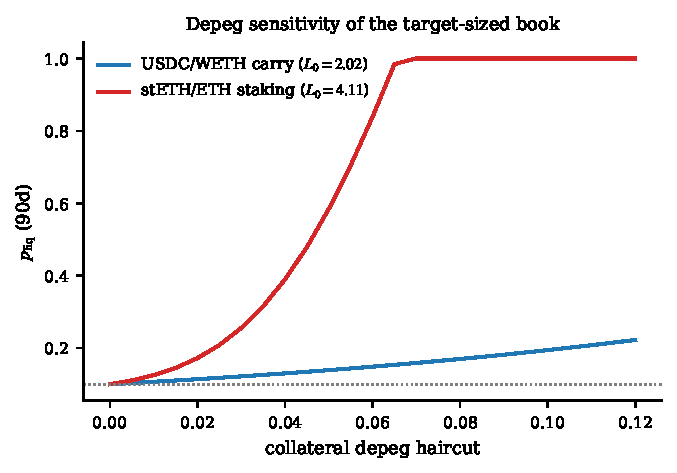
\includegraphics[width=\linewidth]{fig_carry_depeg.pdf}
    \end{column}
  \end{columns}
\end{frame}

% ------------------------------------------------------------
\begin{frame}[plain]
  \begin{tikzpicture}[remember picture,overlay]
    \node at (current page.center) {%
    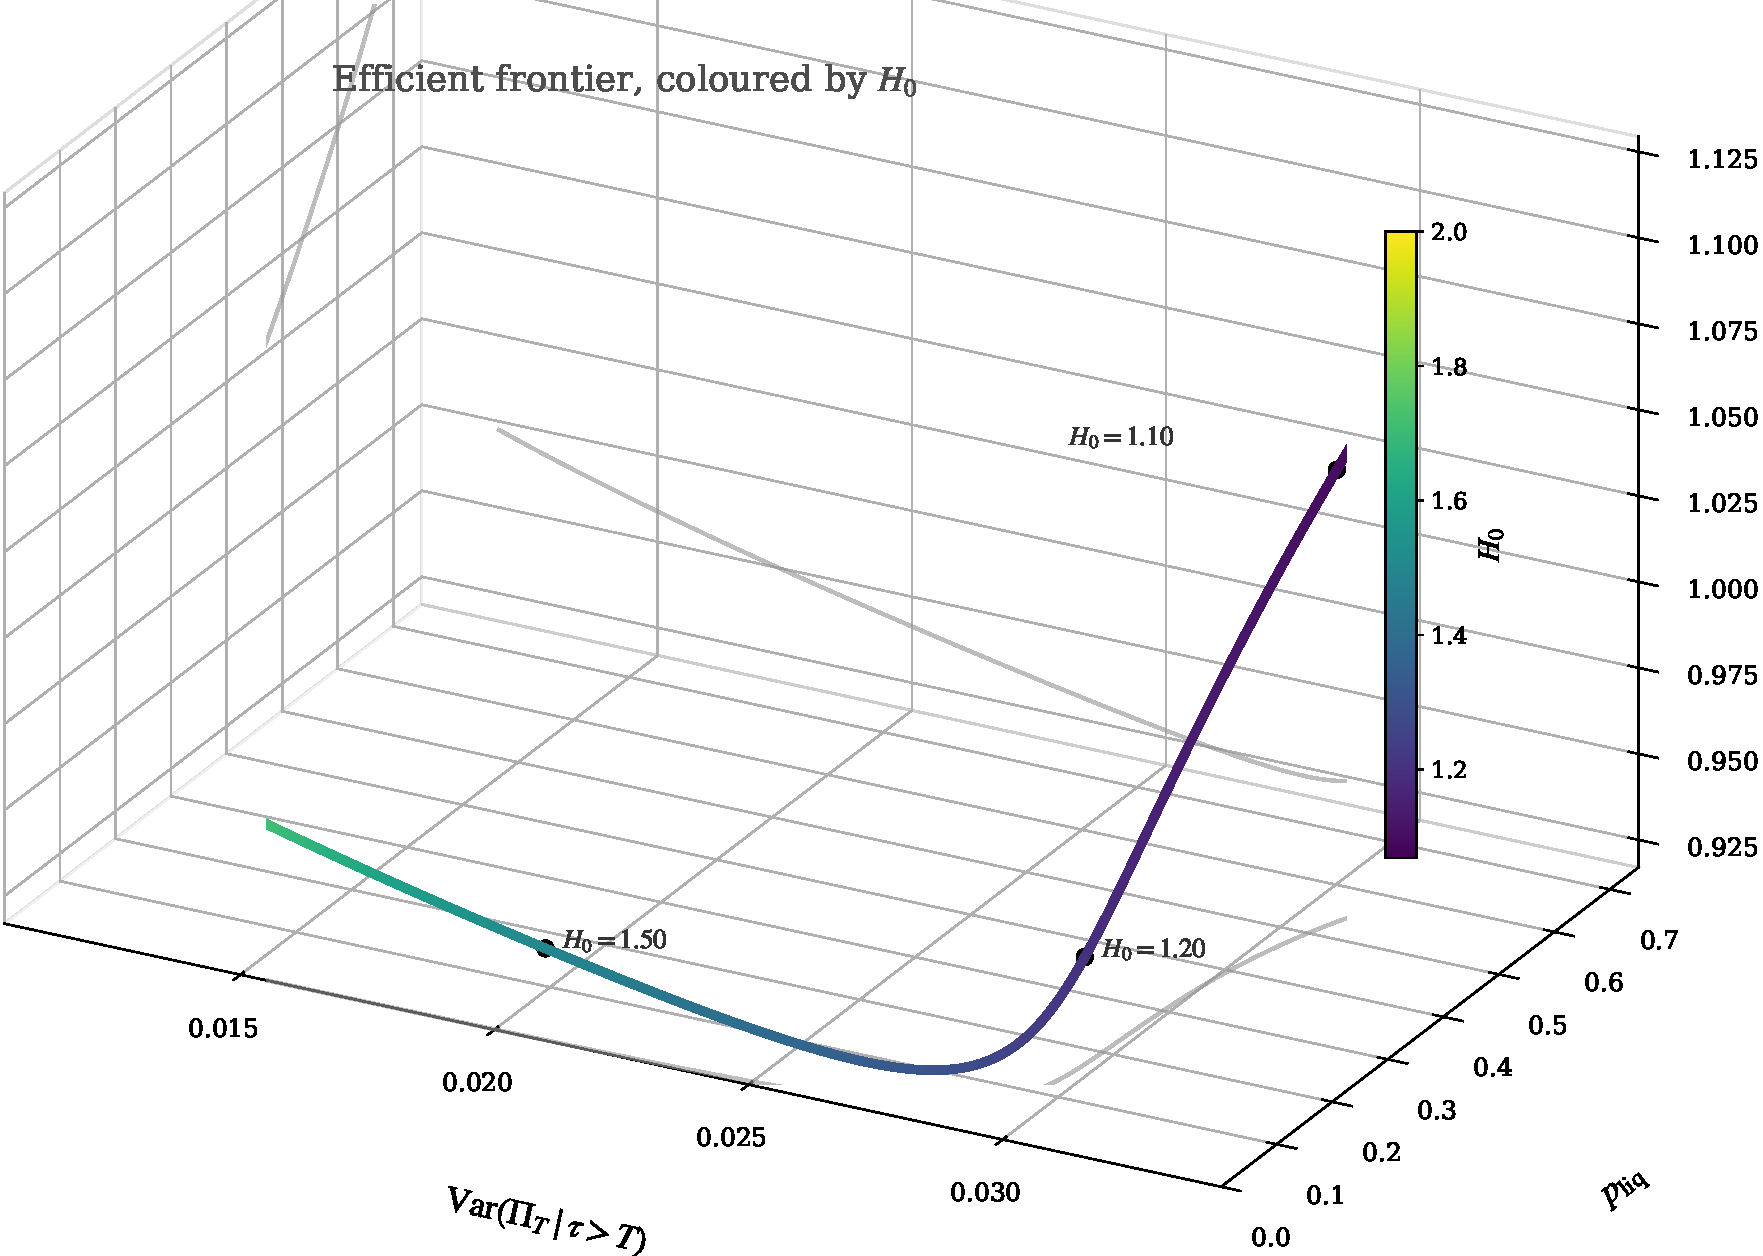
\includegraphics[width=1.06\paperwidth,height=0.98\paperheight,keepaspectratio]{fig_frontier_3d_local.pdf}%
    };
  \end{tikzpicture}
\end{frame}

% ------------------------------------------------------------
\begin{frame}{Conclusions and Discussion}
  \begin{itemize}
    \item DeFi long--short $\rightarrow$ collateral/debt first passage
    \item Central sizing variable: $h_0=\log H_0$
    \item Kou jump diffusion $\rightarrow$ finite-dimensional semi-analytic moments
    \item Fast liquidation-aware sizing; no repeated Monte Carlo
    \item Interest-rate carry $\rightarrow$ per-leg drift shift; interest-bearing books sized with no re-derivation
  \end{itemize}
  \vspace{0.8em}
  \textbf{Ongoing developments}
  \begin{itemize}
    \item Liquidation recovery and dynamic collateral management
    \item \emph{Stochastic} borrowing- and lending-rate modelling
    \item Oracle-delay and execution-slippage overlays
  \end{itemize}
  \vfill
  \begin{center}
    \large Thank you
  \end{center}
\end{frame}

% ------------------------------------------------------------
\begin{frame}{References}
  \footnotesize
  \bibliographystyle{abbrvnat}
  \bibliography{finance}
\end{frame}

\end{document}
